\documentclass{article}


% if you need to pass options to natbib, use, e.g.:
%     \PassOptionsToPackage{numbers, compress}{natbib}
% before loading neurips_2023


% ready for submission
\usepackage[final]{neurips_2023}
% \usepackage[nonatbib]{neurips_2023}


% to compile a preprint version, e.g., for submission to arXiv, add add the
% [preprint] option:
%     \usepackage[preprint]{neurips_2023}


% to compile a camera-ready version, add the [final] option, e.g.:
%     \usepackage[final]{neurips_2023}


% to avoid loading the natbib package, add option nonatbib:
%    \usepackage[nonatbib]{neurips_2023}


\usepackage[utf8]{inputenc} % allow utf-8 input
\usepackage[T1]{fontenc}    % use 8-bit T1 fonts
\usepackage{hyperref}       % hyperlinks
\usepackage{url}            % simple URL typesetting
\usepackage{booktabs}       % professional-quality tables
\usepackage{amsfonts}       % blackboard math symbols
\usepackage{nicefrac}       % compact symbols for 1/2, etc.
\usepackage{microtype}      % microtypography
\usepackage{xcolor}         % colors

\usepackage{listings}       % code
\usepackage{graphicx} %插入图片的宏包
\usepackage{float} %设置图片浮动位置的宏包
\usepackage{subfigure} %插入多图时用子图显示的宏包
\usepackage{amsmath}



\title{CS3308 Machine Learning Homework Project}


\author{
  Your Name
}


\begin{document}


\maketitle


\begin{abstract}
The paper structure is only for reference.
\end{abstract}


\section{Introduction}


\section{Related Work}


\section{Method}

ResNet-50 \cite{he2016deep}.

\subsection{Baseline}

\begin{figure}[H] %H为当前位置,!htb为忽略美学标准,htbp为浮动图形
    \centering %图片居中
    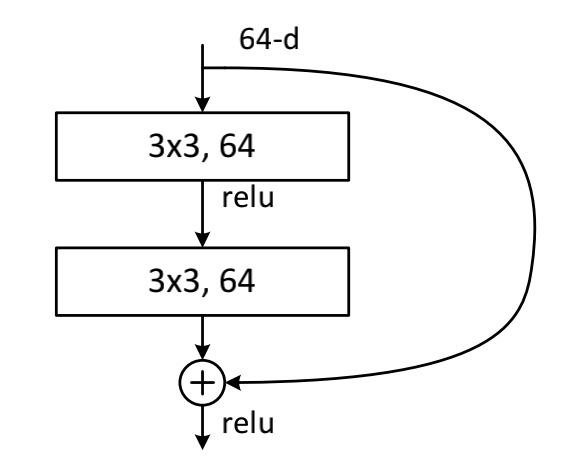
\includegraphics[width=0.5\textwidth]{image.png} %插入图片,[]中设置图片大小,{}中是图片文件名
    \caption{Resnet} %最终文档中希望显示的图片标题
    \label{Fig.img1} %用于文内引用的标签
\end{figure}

\subsection{Ablation}

\section{Experiments}

\section{Conclusion}

\section*{Acknowledgements}

\medskip

\bibliographystyle{plain}

\bibliography{ref}


% \appendix


% \section{Appendix}


% Optionally include extra information (complete proofs, additional experiments and plots) in the appendix.
% This section will often be part of the supplemental material.


\end{document}